\documentclass[13pt, a4paper, twoside]{article}
\usepackage[utf8]{inputenc}
\usepackage{geometry}
\usepackage[czech]{babel}
\usepackage{chemformula}
\usepackage{chemfig}
\usepackage{enumitem}
\usepackage{fancyhdr}
\usepackage{caption}
\usepackage{setspace}
\usepackage{float}
\usepackage{multicol}
\geometry{legalpaper, margin=1.05in}
\pagestyle{fancy}
\lhead{\Large Šárka Doležalová, skupina 6}
\rhead{\large 10.12.2020}
\begin{document}
\begin{center}
    \Huge
    Úloha 4: Stanovení teploty tání
\end{center}
\onehalfspacing \large
\section*{Zadané úlohy}
\begin{enumerate}
    \item Stanovte teplotu tání předložených vzorků A a B. Na základě naměřených hodnot určete,
    o jaké látky se jedná.
    \item    Stanovte teplotu tání směsí látek A a B s hmotnostním obsahem látky A 10, 25, 50, 75
    a 90\% (obsah látky B je komplementární, tj. 90, 75, 50, 25 a 10 \%).
     
\section*{Teoretiký úvod}
\subsection*{Práce s bodotávkem}
Existují 3 typy bodotávků. Skleněný naplněný látkou s vhodnou tepelnou kapacitou, dříve užívaný pro látky s nízkou teplotou tání. Kovový, dobře vodivý, pro teploty s vyšší teplotou tání. A elektrický, automatizovaný, který používáme dnes.
Postupujeme tak, že vzorek napěchovaná v tenkostěnné kapiláře vložíme do vyhřívané lázně bodotávku. Na displeji se ukazuje momentální teplota v lázni a my mezitím pozorujeme lupou látku v kapiláře do jejího roztátí.

\section*{Postup}
Bylo naváženo 0,0930 g vzorku A (vzorek 46), který byl vložen do třecí misky, kde byl pečlivě rozetřen a poté na hodinovém sklíčku uložen do exsikátoru. To samé bylo zopakováno se vzorkem B (vzorek 42), ale bylo ho naváženo 0,1085 g. Z rozetřených vzorků, bylo do malých vialek odváženo podle následující tabulky.


Navážené směsi, byly znovu rozetřeny v třecí misce a byly jemi naplněny jimi naplněny vždy 2 kapiláry. U vzorků byla stanovena teplota tání, nejprve u čistých látek poté u směsí.

\section*{Naměřené hodnoty}
\begin{figure}[H]
    \centering
    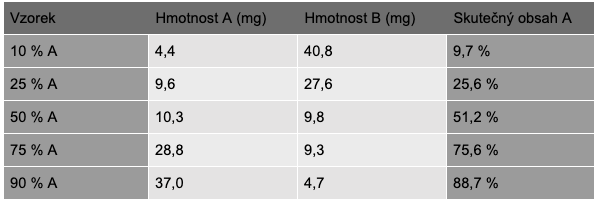
\includegraphics[width=7in]{uloha_4_tab_1.png}
    \caption*{Tabulka navážených vzorků a jeich procentuální zastoupení}
\end{figure}



\begin{figure}[H]
    \centering
    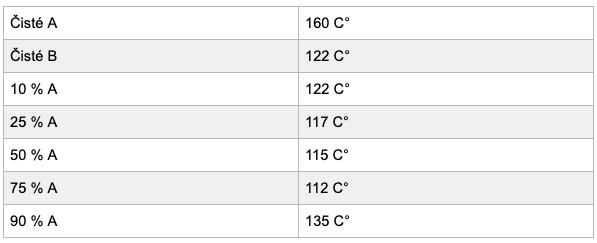
\includegraphics[width=7in]{uloha_4_tab_2.png}
    \caption*{Tabulka teploty tání při měření s $5^{\circ}C/min$}
\end{figure}

\begin{figure}[H]
    \centering
    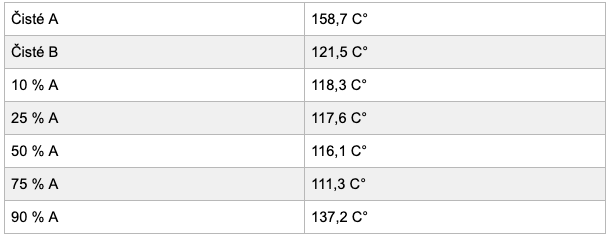
\includegraphics[width=7in]{uloha_4_tab_3.png}
    \caption*{Tabulky teploty tání při měření s $1^{\circ}C/min$}
\end{figure}

\subsection*{Graf}
\begin{figure}[H]
    \centering
    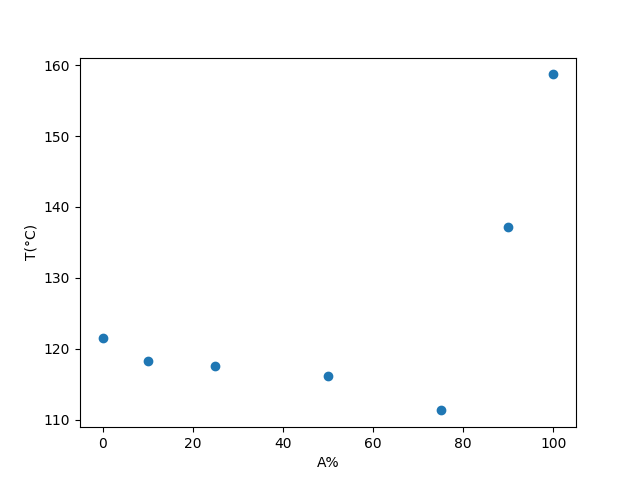
\includegraphics[width=5in]{teplota_tani_graf.png}
    \caption*{Graf teploty tání při měření s $1^{\circ}C/min$}
\end{figure}

\section*{Závěr}
Porovnáním teplot tání jsme určili, že vzorek 46 byla kyselina salicylová vzorek 42 byla kyselina benzoová.




\end{enumerate}
\end{document}